\documentclass[journal, a4paper]{IEEEtran}


\usepackage{graphicx}   
\usepackage{url}     
\usepackage{multicol}
\usepackage{amsmath}  
\usepackage{graphicx}
\usepackage{xcolor}
\usepackage[export]{adjustbox}
\usepackage{verbatim}


\begin{document}
    \twocolumn[
    \begin{@twocolumnfalse}
	\title{Spectral Image Clustering Segmentation}
	\author{Jericho O'Connell, Kevin Murphy, Kris Iniewski, and Magdalena Bazalova-Carter }
	\maketitle

\section{Abstract}

    \newline
    \end{@twocolumnfalse}]
\section{Introduction}


\PARstart{S}pectral imaging remains an unexplored imaging modality for multiple reasons. Firstly the price of spectral detectors is a large barrier to the clinical implementation. Secondly the applications where spectral imaging outdoes single energy and dual energy imaging are not well defined. Although there has been much interest in spectral CT in medicine it is often seen to have only small benefits as compared with dual energy CT in the same application. 

In this work we examine spectral imaging as compared to dual and single imaging in the application of segmentation. A comparison is made of the performance of unsupervised segmentation algorithms is performed on experimental images acquired using a Redlen (redlen industries ...) spectral detector on a phantom composed of a variety of materials as well as images aquired of these same materials embedded in chicken breast.

\section{Materials and Methods}

\subsection{Imaging setup}
\begin{center}
\begin{figure}[htbp]
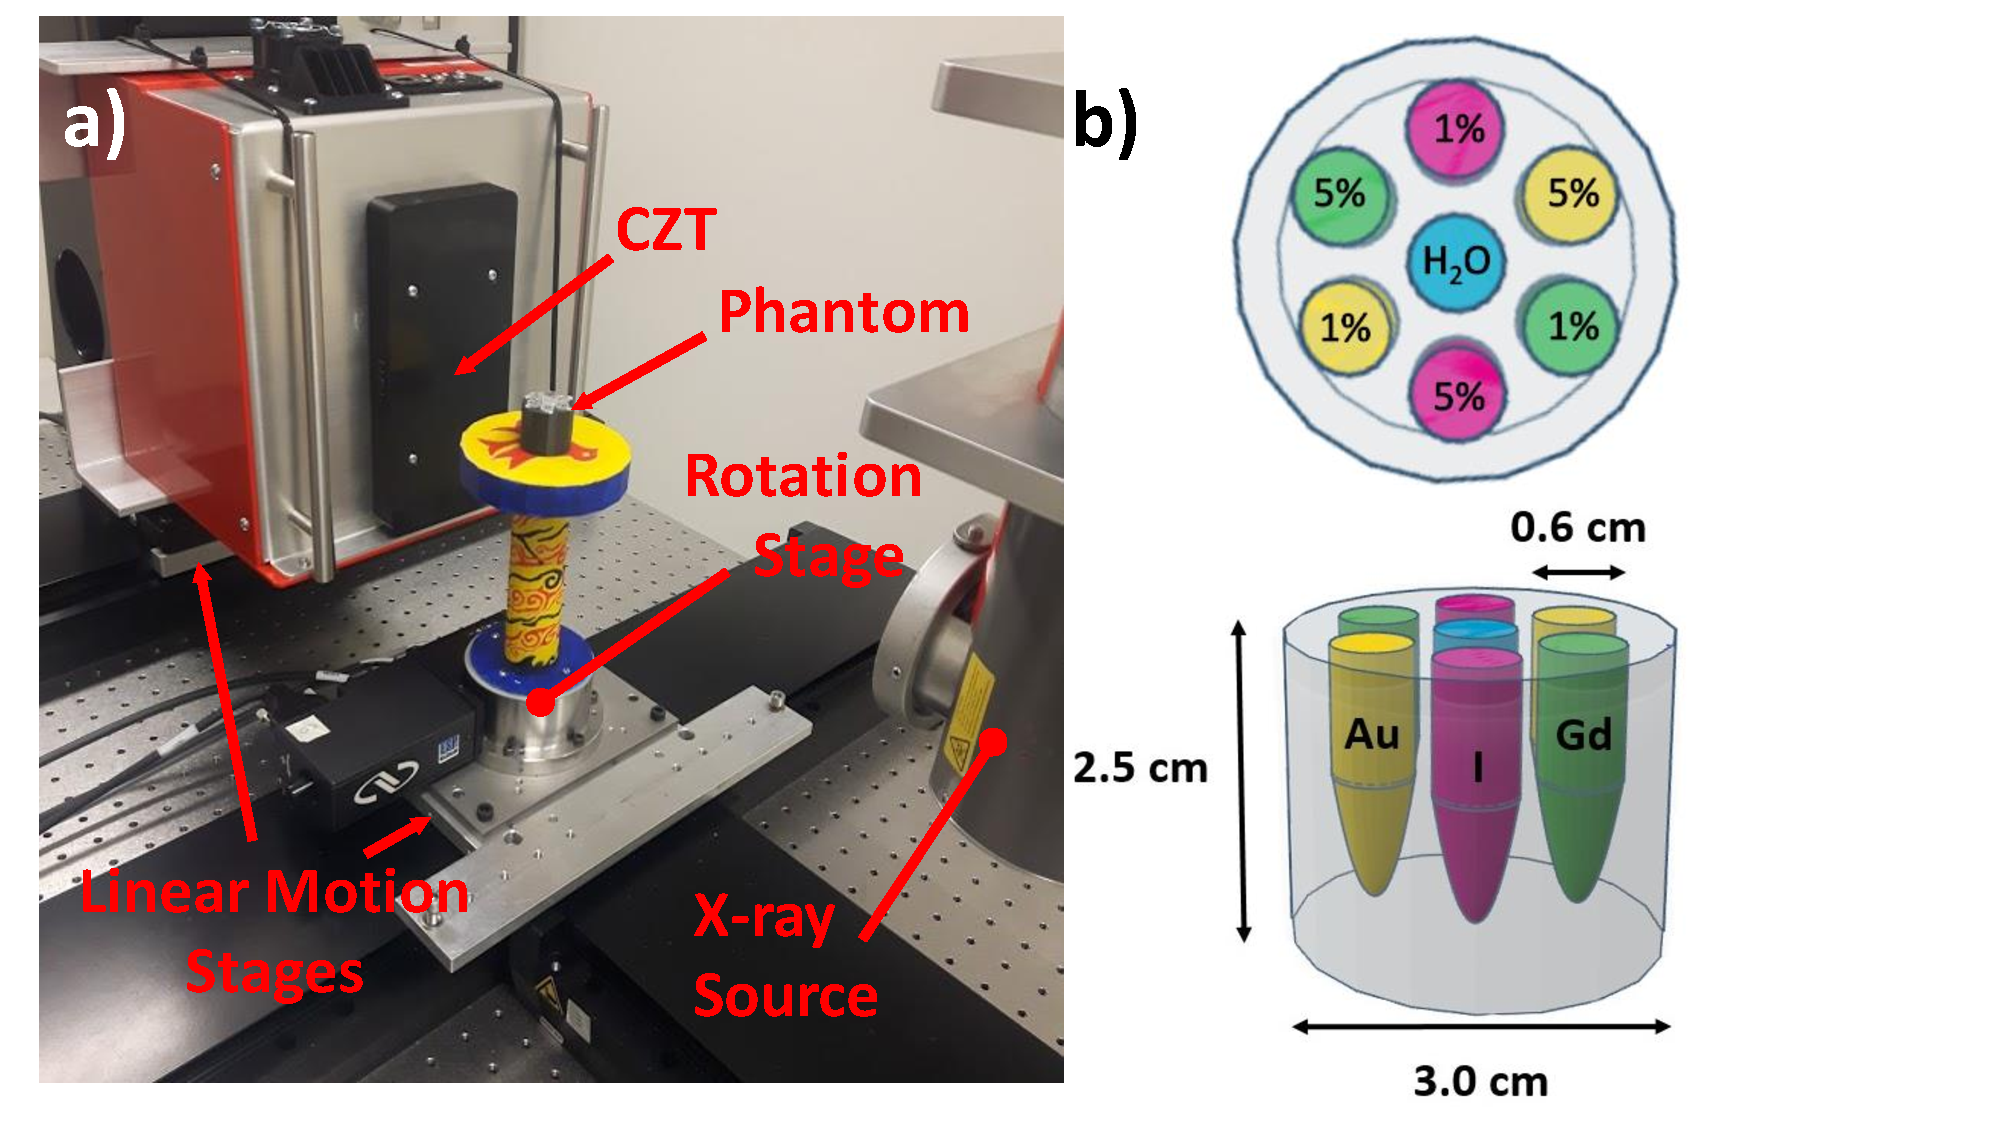
\includegraphics[width=\linewidth]{PhantomOrientation.pdf}
\caption{a) Lab set up for Spectral CT data acquisitions, with components labeled.  b) Contrast phantom holder with layout of concentrations for each contrast agent. }

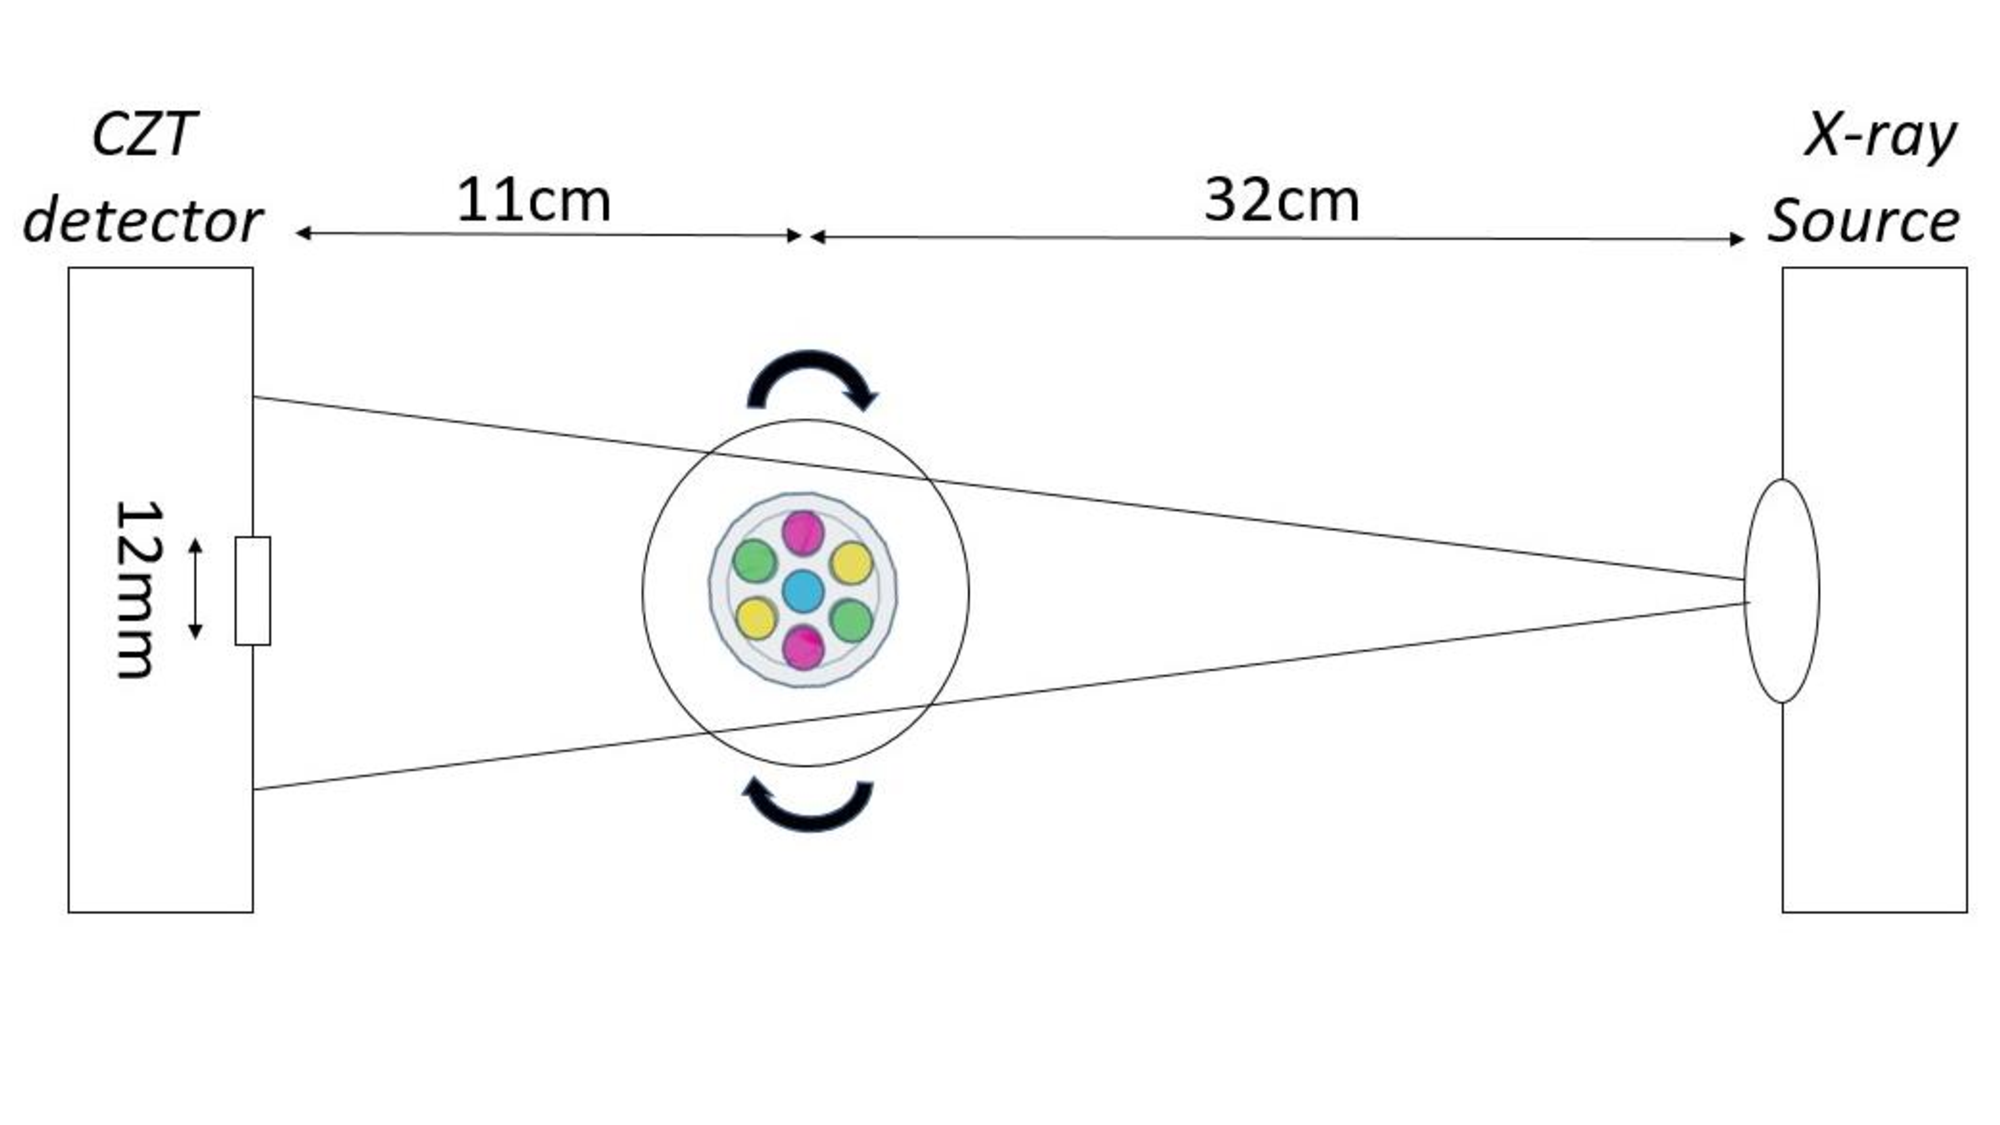
\includegraphics[width=\linewidth]{LabSchematic.pdf}
\caption{CZT spectral CT design schematic}
\label{imagingsetup}
\end{figure}
\end{center}


\subsection{Data Aquistion}
X-ray scans were performed on a PMMA phantom with 5 contaminates (steel, glass, plastic, polypropylene, and PFTE) as well as chicken flesh with various contaminates (bone, cartilage, fat, plastic, wood, glass, rock, steel, and aluminum).

Data was acquired using a CZT detector with a 8$\times$12 mm imaging array from Redlen Technologies. The 330 $\mu$m pitch high-flux CZT detector is 2mm thick and is able to operate at 250 $\frac{Mcps}{mm^2}$ without any signs of polarization. Travel Heat Method (THM) was adopted by Redlen Technologies when growing the CZT crystals used in the detector. These crystals were placed in a sensor that is connected to a photon counting ASIC which operates at rates of up to 62.5 $\frac{Mcps}{channel}$. This ASIC communicates with an external PC though LVDS I/Os via a programmable FPGA. The energies of photons incident with the detector are sorted into six energy bins by the ASIC. In the case of this experiment the energy bins were set to 16-33 keV, 33-41 keV, 41-50 keV, 50-90 keV, 90-120 keV, \& 120< keV.

The detector and X-ray source were both mounted on vertical and horizontal linear motion stages from Newport Corporations. These stages were oriented perpendicular to each other to allow for easy navigation while imaging the phantom, which was mounted between these two stages. The X-ray source used was a module XRS-160 from Comet Technologies. 

The PMMA phantom block as imaged in figure (1.C) was placed on the stage and the 3 smallest contaminates of each material were imaged. To image these contaminates each at different heights, the CZT detector and X-ray source were moved vertically in a uniform manner allowing for each material to be centered without any motion of the phantom block itself. Following the first round of data acquisitions a second block of 18mm PMMA was placed in front of the phantom block and images were acquired to determine the depth at which each contaminate could be visualized. 

In the case of the chicken flesh, each contaminate was able to fit in a phantom holder alongside the chicken. This block was placed on the stage and was able to be imaged in one scan per contaminate. 

Air scans were completed for each data acquisition and could then be processed using MATLAB (The Mathworks, Natick, MA) for image reconstruction and CNR calculations for each contaminate. During all scans the X-ray tube was using a cone beam operating at 1mA, 120 kV, with a 1mm focal spot. 

% \begin{figure}[htbp]

% \includegraphics[width=\textwidth]{FullFigure.jpg}

% \caption{A) Shows an image of the lab after data was acquired with different components as labeled. B) Is a schematic of the lab with distances from source to detector labeled. C) The layout for the phantom used with sizes of contaminates as labeled.}
% \label{figcali}
% \end{figure}

\subsection{Dimensional Reduction Methods}

As described by (???) segmentation follows multiple steps includding preprocessing, dimensional reduction, clustering and postprocessing. Dimensional reduction methods were used in this work to both help visualization and to increase class seperation in an effort to make the clustering more successful.

\subsection{Clustering Methods}



\subsubsection{Number of Clusters}

Many of the algorithms that are shown below include a parameter that specifies the number of clusters that will be created by the algorithm. This is a problem as the ideal clustering method would have the option of assigning all of the points in an image to the same class, which should be the default case in non-desctructive testing. However, there are methods that accomplish this that are specific to each clustering method discussed. So as a first step we will examine all of the clustering algorithms based on their performance on the given two class clustering problem of the phantom and then select the best model and discuss how it asses what number of clusters it should use as input to the algorithm.

\subsubsection{Performance Metric}

The performance metric used to evaluate the clustering method was the V-score as defined by (???). The V-score was used due to its intuitive nature. A V-score is the harmonic mean of the homogeneity and completeness score of the clustering as compared to a ground truth. The ground truth used were manual segmentations of the image. A clustering is said to be complete ($c$) if all the data points of a given class are in the same cluster. Conversely, a clustering is said to be homogeneous ($h$) if all clusters contain data points of only one class. These metrics are defined in terms of conditional entropy as

$h = 1 - \frac{H(C|K)}{H(C)}$

$c = 1 - \frac{H(K|C)}{H(K)}$

Where $C$ is the classes and $K$ is the cluster assignment, and $H(C|K)$ is the conditional entropy of the classes given the clusters assigned and is defined as

$ H(C|K) = - \sum_{c=1}^{|C|} \sum_{k=1}^{|K|} \frac{n_{c,k}}{n}
          \cdot \log\left(\frac{n_{c,k}}{n_k}\right)$

and $H(C)$ is the **entropy of the classes** and is given by:

$H(C) = - \sum_{c=1}^{|C|} \frac{n_c}{n} \cdot \log\left(\frac{n_c}{n}\right)$

\subsubsection{K-means}

The first clustering method implemented was k-means clustering. K-means was implemented using the k-means++ algorithm of (???). K-means was fit using a value for the number of clusters $k$ defined through the use of silhouette analysis. Different distance metrics were used, however none of the distance metrics tried improved performance over the squared euclidean distance, thus squared euclidean distance was used as the metric.

\subsubsection{Mean Shift}

A mean shift clustering was also applied to the data. The mean shift algorithm as described by (???) does not take as input the number of clusters to be found in the data. The bandwidth was estimated using the scikit learn method for estimating bandwidth which uses a it is determined using a heuristic based on the median of all pairwise distances. A radial basis function (RBF) kernel was used in the clustering.

\subsubsection{Spectral Clustering}

Spectral clustering first described by (???) is a method that takes the spectrum of the similarity matrix, a matrix constructed which holds the pairwise similarity of points in the dataset using a defined distance metric. In this work the multiple distance metrics were used to construct the similarity matrix. As with k-means the spectral clustering algorithm takes as input the number of clusters. This is problematic as the ideal clustering method would have the option of assigning all data points to one class.

\subsubsection{Ward Linkage Hierarchical Clustering}

Although multiple heirarchical clusterings were tried using different linkages, ward clustering was decided as the the superior clustering method as it is the most robust with noisy data. First described by (???) heirarchical clustering builds nested clusters by starting with every point as a single cluster and iteratively merges or splits clusters based on some distance metric. For Ward clustering the clustering minimizes the sum of squared distance as until convergence. This is the same metric as k-means clustering save with agglommerative approach rather than a centroid approach. Two other parameters included in the algorithm are the linkage and conectivity. The connectivity governs the 

\subsubsection{Birch}

Another form of heirarhcical clustering, the Birch clustering algorithm, a stable and fast algorithm, has the ability to cluster large datasets with only small amounts of memory as well as the ability to discard outliers. These features are not included in Ward Linkage Hierarchical Clustering. Birch requires the desired number of clusters as an input.


\section{Results and Discussion}

\subsubsection{Dimensional Reduction Results}

The three different methods for dimensional reduction are compared in figure (???), the dimensional reduction methods were compared in terms of the v-measure of the resultant clustering. All of the clusterings were performed on two dimensional data after the dimensional reduction step. The performance of the algorithms without the dimensional reduction step was also performed for comparison to justify the use of dimensional reduction.

The PCA dimensional reduction has superior performance when using the GMMs and good performance on all other algorithms. This was taken as a result of the linear transformation performed under the PCA which preserved the gaussian structure resultant from the photon statistics of the imaging process. Non-linear methods such as tSNE, which can be seen in figure (??) , resulted in good separation of the data especially when the position data was added as a feature as seen in the figure. One can see how the background of the image when coupled with its position data is embedded as a rectangular cluster in the tSNE scatter plots, however tSNE being non-linear created a large separation between the partial volume pixels and contaminant pixels. This results in lower V-scores ever when coupled with an algorithm that clusters the data perfectly such as HDBSCAN.

NMF dimensional analysis was also performed on the data. Although on average the results had lower V-measures than the PCA or no dimensional reduction, there were some cases that defied this trend. As can be seen in figure (???) the hard materials when decomposed with NMF and the GMM algorithm resulted in the best fit even when compared to the dual and single energy cases which will be seen in the next section.


\subsection{Clustering Results}


The results of the clustering can be seen in the scatter plot. One can see that the data is clustered in an overlapping roughly Gaussian blob for the soft tissues. For the hard tissues one can see that the data is spaced out over a few blobs, one large blob that contains the background pmma and multiple sparser foreground blobs that indicate the different inserts.

The attempts to classify the data were largly successful with almost all algorithms classifying the largest inserts correctly and worse results on the smaller inserts and added varying amounts of error on the partial volume pixels. One can see that the methods which used euclidean distance (kmeans, mean-shift, ward, Birch) has limited success when dividing the clusters. The largest v-score generated from these methods being (???). The hdbscan algorithm has some success binning the algorithms, with a winning combination for dbscan being the use of tsne as a dimensional reduction method before clustering using DBSCAN as this clearly seperates the data in visible clusters as mentioned in the previous section. However these clusters are not necessarily homogenous nor complete, as can be seen by the v-score assigned to these clustering methods.

Spectral clustering produced higher v-measure than the euclidean distance based metrics as well as dbscan and Birch on the soft materials. On the hard materials spectral clustering produced similar results. In fig (???) one can see that a good algorithm is characterized by being able to form a globular cluster around the background pmma and hold the outliers from this cluster as the members of the second class.

This is best described by the most successful algorithms the Gaussian Mixture Models which had the highest V-scores overall for all materials. Successfully forming a background cluster and assigning the outlying points to the second cluster the GMMs were best able to optimize based off of the gaussian shape of the data.

\subsubsection{Single and Dual Energy Comparison}

In fig (???) the performance of the clustering is compared between the single energy case, which sums the counts in all of the bins to make one image and a dual energy case which creates two bins by summing the photons in bins 1-3 and 4-5 to form two images. 

The single and dual energy cases show improvements in performance relative to the spectral imaging looking at the hard tissues. This is expected as the greatest variance in the image is due to the density difference of the two materials, thus the data is linearly separable in the one and two dimensional image spaces of single and dual energy imaging. In the softer materials the spectral imaging superior V-measures compared to the single energy case as would be expected since these materials cannot be linearly separated through their attenuation alone and the energy dependence of the attenuation, acquired through spectral imaging, creates a higher dimensional set of features that can be clustered more easily. More surprising perhaps is the improvement of the V-measure in the spectral case as compared to the dual energy case in which both imaging methods contain information about the energy dependence. Previously it was believed that spectral imaging has little improvement over dual energy in cases such as this ref(???).

One other anomalous result is the effectiveness of NMF coupled with GMMs on the hard materials



\bibliographystyle{IEEEtran}
\bibliography{IEEEabrv,spectralCT}
%\begin{thebibliography}{1}
%    \bibitem{}
    
%\end{thebibliography}
\end{document}


https://www.overleaf.com/8631237895wkwqdddspdtkhttps://www.overleaf.com/8631237895wkwqdddspdtk